\chapter{Motivation}\label{ch:motivation}

\begin{figure}[h]
    \begin{center}
    {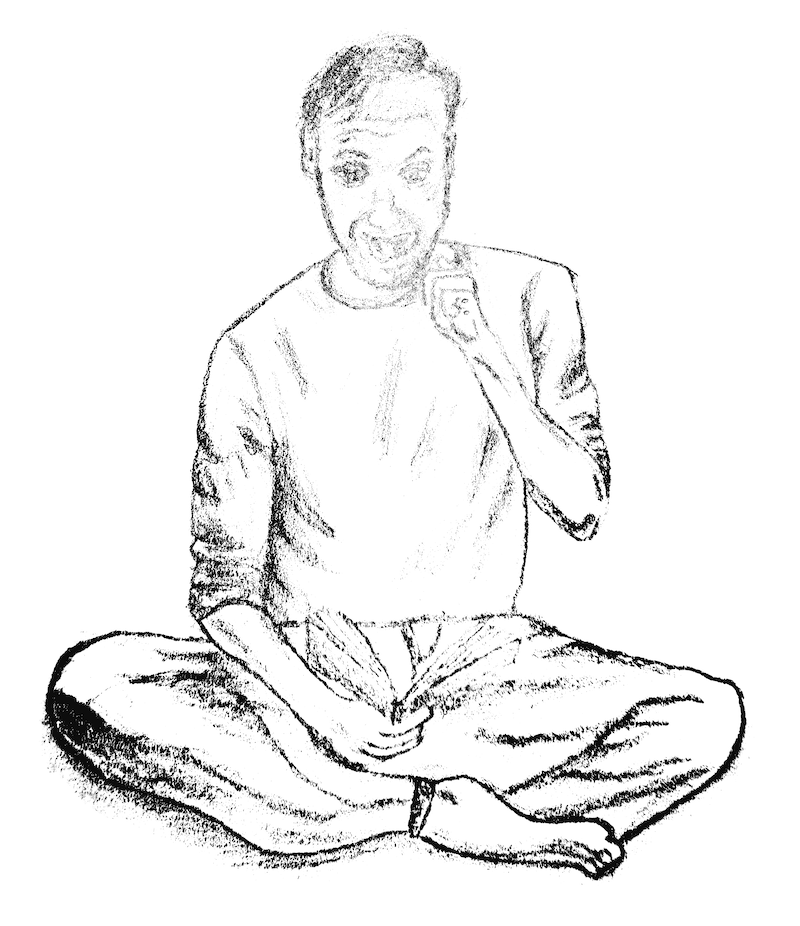
\includegraphics[width=0.3\paperwidth]{images/testpic}}
    \end{center}\label{img:motivation}
\end{figure}

\begin{displayquote}
    ``\textit{If meditation is the process of being in the present moment, in the so-called here-and-now, then Contact Improvisation is the highest form of meditation.}''
\end{displayquote}

Besides for the obvious reason for dancers to expand their skill-set, non-professionals are most likely to start with CI for either simply the \textbf{pleasure} of doing it -- as it is fun --, or sometimes as well for \textbf{personal development} purposes.
We all come to doing the same things sometimes for very different reasons, and all of them are valid, and some of them might be suboptimal as other methods might be more effective in attaining your goals.

This section might get you inspired to start, or even motivate you further to deepen and dedicate more of your life into this ``useful'' art.
The given reasons might all be indeed valid, yet they are not, and should not be the main reason, the main intention to do CI, there are simply co-existing.

\section{The Power of Touch}\label{sec:the-power-of-touch}

The tactile experience is most prominent during practicing CI. To be specific, it's the activation of nerve fibers in the skin, the so called \textit{C tactile afferents}, through gentle and slow stroking with body-like temperature.
A ``warm touch'' leads to the release of \textbf{serotonin}, a hormone which makes us feel happy, regulates our emotions and associated with sympathy and interpersonal affection; ``cold touch'' is experienced when being socially excluded, as the skin temperature decreases.
Such a touch will increase activity in the insular brain region that is responsible for interoception, which is perception of the current body state and facilitation of the sense of self.
This touch, which can be soft to slide, or deep to the bones, is used to establish a nonverbal, two-way dialogue process, a form of \textbf{communication}.

This kind of touch reduces stress (lowered cortisol levels, which is a biomarker for stress-related diseases), increases oxytocin levels (attachment, connectedness) and lowers blood pressure.
If a person lacks touch, disorders like depression, a distorted body image, low self-esteem and heightened aggression and self-injurious behavior might occur.
Touch releases endogenous \textbf{opioids}, which make us feel relaxed, good, and more resilient.
It counteracts a feeling of loneliness and isolation, which is the case in many forms of mental disorders --in the UK alone, about 54\% (among 40,000 participants) want more touch in their lives.
We are living in a low-touch society where mistrusting strangers became a default.

Yet, touch needs to happen with \textbf{consent} to be experienced as something positive.
To want to touch, and want to be touched.
Respecting each other's \textbf{boundaries}, and the possibility to step out of touch at any given moment.
A good CI facilitator will address those things, by, for example, introducing ``yes/no-exercises'', and safety rules at an event.
Especially beginners, who are easily overwhelmed by touch and lost trust in others, due to previous bad experiences, can benefit from a gender-based group and sharing circles in a safe space to reflect upon.

\section{Psychological Benefits}\label{sec:psychological-health-benefits}

CI has been reported to have \textbf{positive effects} on stress relief, relaxation, well-being, happiness, joy, connectedness, empowerment and feeling more fearless.
Also leading to a clearer experience of a ``sense of self'' and the body; being more aware of one's own existence.

The massage effect of ``sharing weight'' seems beneficial against anxiety, depression, ADHD, eating disorders (``better sense of one's own body''), autoimmune diseases, chronic fatigue syndrome, and more.
It also helps with the activation of the parasympathetic nervous system -- ``\textit{rest and digest}''.

As the attention is attracted to the ``shared zones of contact'', it brings us to the present moment, and thus becomes a \textbf{mindfulness practice}, distracting us from stressful thoughts.
There is no intention to reach a certain goal, but simply \textbf{exploring} movement and touch itself.
This requires us to be attentive, aware and present.

Finally, the personality gets strengthened, by being more aware of one's own \textbf{needs}, and distinguishing oneself from the others.
\textbf{Patterns} can be broken, not only in movement, but also in behavioral and cognitive patterns, and a positive impact in resilience-building might occur.

\section{Social Bonding}\label{sec:social-bonding}

CI helps us \textbf{to relate} better to others, to create stronger social connections, \textbf{to connect} to other people and bodies.
At the beginning, this connection with others might not be so present, as we focus on the technicalities (the bodies, not the peoples); the focus resides on creating a piece, not a community.
The experience of giving and receiving support via ``sharing weight'' for example.
The sensation goes beyond the pure physically into the psychological and emotional realm.
To trust each other, to feel safe again; presenting our vulnerabilities and instabilities, ultimately leading to a state of \textbf{safe intimacy}.

It has been reported that the following experiences during a dance can emerge: playfulness, surprise, curiosity, flow state, feeling free, being alive, vitality, nourished, energized, connectedness, trust, closeness, deep communication, safe, secure.
The sensation of connectedness feels like being a new ``third entity'', as it is not clear who gave the impulse to move in a certain way.
``\textit{By feeling the other person more, I feel my own boundaries better, and thus I feel myself more, feeling more home in my own body.}''
Yet, negative sensations might occur as well, of course, like boredom, insecurities, doubts, exhaustion, strenuous and being at one's own mercy.

It can connect people from all backgrounds, as we all have the \textbf{same body}, being equalized, moving in space, independent of age, gender, sex, belief, religion, or color.

\section{Soft Skills}\label{sec:soft-skills}

Through the practice of CI, many soft skills are also trained and enhanced, such as teamwork, problem-solving, communication, interpersonal skills, adaptability, dependability, and creative thinking; which are all not only important in our personal, but also in our professional life.

In \textbf{teamwork}, we achieve a common goal while supporting the strengths of others.
While we dance with a partner, we are looking and seeing where all the other couples are and moving through and around us.
Our goal is to have an enjoyable dance, while letting others have one too.
By literally supporting our partner, and choosing together how to navigate the space, we form a small team.
The so-called \gls{bigspace}, the heightened awareness of all the people within a room, we all pay attention to each other, forming a big team.

Every contact is a little kinetic puzzle which requires \textbf{problem-solving} skills.
Like watching two improvisation actors saying ``Yes, and \ldots'' a little too often, and you wonder how they will get out of that; yet with CI, the very same happens just physically.
Navigating through space, while watching not to bump into others or hit the wall, and all of that while maybe your partner is trying to balance on your body.
All of those puzzles need to be somehow solved at the same time.

Good \textbf{communication} skills require deep, active listening;
yet with CI, we mostly stay in silence, so the attentive listening happens only non-verbally with the whole body.
There is never an agenda, a script, or a predefined choreography.
No one knows upfront what's going to happen, who is going to initiate what.
Yet surprising as it sounds, with good enough listening skills, there will always be clearly communicated what will happen in the immediate next moment; by simply listening and responding.

\textbf{Empathy} is an essential part of interpersonal skills, which is practiced in CI by ``feeling the earth through our partner's feet''.
Although you might not know anything about your current dance partner, through this interaction you will experience so much about how they live in this world, as: ``\textit{Bodies speak beyond words}''.
It's not only the obvious, physical characteristics like size or weight, but also the techniques being most often used and general movement choices which tell us a story.
Through this, we might not be aware of facts like country of origin or the family status, but in a different dimension we still get to know the person.

There is such a vast variety in Contact Improvisation dancers that \textbf{adaptability} becomes actually a significant skill which gets acquired very fast due to its necessity.
Obviously, the amount of weight you can share with your partner needs to be adjusted.
The differences in height make certain techniques, such as lifts, more or less easy, or even impossible.
And of course, the level of experience with body practices in general, and CI specifically, requires you to adapt to what's there - and possible - at the moment.

An interesting contradiction in CI is, that on the one hand you have to be able to completely rely on your partner, building up trust (\textbf{dependability}), and on the other hand to always stay within your own center, being able to catch yourself at any given moment (\textbf{self-reliance}).
Always take care of yourself, while being hyper-aware of where your partner is, how he is moving and where he is going;
and also knowing what the other people are doing in the room, having one's awareness spread throughout the \gls{bigspace}.
Bear also in mind that you can't know what's going to happen, predictions are impossible due to the improvisation nature of CI, thus the name.

\section{Other Motivations}\label{sec:other-motivations}

Definitely, there are benefits in the area of personal and social growth.
Maybe it could be even considered a philosophical, mental, and/or \textbf{spiritual practice}.
Its slowness resembles some meditative state and its fastness to stay in the flow, in the zone, in order to ``survive''.
Like ballet, where dancers stay in the zone of awareness, a meditative state, by doing, for example, a plié for more than 15 minutes.
Just in CI, instead of pliés, we do the \gls{smalldance}.

As a \textbf{body-oriented practice}, it will refocus your mind more to the body, the physical sensations.
It's not about getting out of your head, but more being able to use your thoughts and direct them like a spotlight.
In case you are not there, fully present with all your senses, attention and thoughts, the dance will tell you by bumping and falling.

A very pleasant side effect is that it can also act as a form of \textbf{workout}.
By this, we avoid having to go to the gym and have much more fun in the studio playing with each other.
Some people run to lose weight, we go dancing.
``\textit{Some people lift weights, we lift bodies.}''

It sparkles \textbf{curiosity} in us to explore the exercises further.
For some it is a starting point of such exploration, whereas less than half stay with CI, others continue somewhere else.
The love for the capacity to move in a different and totally new (path)way.
These new pathways are often explored due to its improvised nature that is part of the dance improvisation world, without any choreography, which often leads to the loss of the reason why we are doing it, and simply following someone else's idea without questioning it.

On a much deeper level, it is also a way to \textbf{handle life}, in a comfortable, safe environment.
A place to see humanity, or better: animality.
In a good kind of way, a monkey kind of way, which is very much fun.

Lastly, you will also gain some more \textbf{insights} into yourself, knowing more about your personal boundaries and tolerance for risk.
How you want to be treated, and how to be heard.
What your tendency is in regard to taking over a conversation.
Realizing that you are not as heavy as you imagined yourself to be.
You learn to be vulnerable and to trust others with your vulnerability: ``\textit{When I fall, will you catch me?}''

\section{Society and Touch}\label{sec:society-and-touch}
%%%%%%%%%%%%%%%%%%%%%%%%%%%%%%%%%%%%%%%%%%%%%%%%%%%%%%%%%%%%%%%%%%%%%%%%%%%%%%%%%%%%%%%%%%%%%%%%%%%%%%%%%%%%%%%%%%%%%%%%

Let's take a look at CI being embedded in the bigger picture of society and culture.
How they mutual \textbf{impact} and shape each other, and what position CI might have in our current world.

In a very strictly gender-role based society, where usually no same-sex touch is permitted, CI would have big problems becoming popular.
Our Western World is seen as a non-touch society, yet there are bubbles where it is allowed and even encouraged; e.g.\ couple dancing, although not the entire body but only holding or embracing arms and the back.
Because of the lack of (connection via) touch, and us being basically \textbf{social mammals}, these bubbles might get more and more attraction somewhere in the (near) future.
Especially people who don't have others close to them, like relatives, loved ones, partners, or other people with whom one can share physical intimacy like cuddling, or in those extreme circumstances like during COVID-19, we feel again that basic human need for touch, also called ``skin hunger''.
But be aware that this is not the aim of CI!
It's just a very nice additional \textbf{side effect}, but not it's declared goal or intention.
People who only come for that side effect, won't stay long.
There are plenty of other places where you can get touch for that purpose; CI is not being one of them.

Using CI in order to ``heal the world'' seems a bit\ldots let's say utopian, or maybe even naive.
This approach is more well-fitted for younger people, with lots of enthusiasm, and still being overly eager, and that eagerness comes because CI can indeed change one's life.
But one thing is for sure: The more we \textbf{spread} CI, the better.

\begin{displayquote}
    ``\textit{If everyone would do CI, there would be no wars anymore, and it would be the end of capitalism}'', says the young.
\end{displayquote}

\begin{displayquote}
    ``\textit{CI is a very, very rich, beneficial and amazing dance form, and it might not change the world, but it did change me}'', says the old.
\end{displayquote}
